\section{Skup podataka za treniranje}
\label{sec:dataset}

Prvi korak u izgradnji sustava koji koristi bilo kakav tip modela strojnog učenja
je odabir i priprema prikladnog skupa podataka na kojem će se taj model trenirati.
Budući da je cilj sustava prepoznavanje govornih naredbi (eng. keyword spotting),
savršen otvoreni skup podataka je skup za treniranje prepoznavanja ograničenog
skupa naredbi \cite{speechcommandsv2}. Riječ je o skupu koji
se sastoji od oko 105000 zvučnih isječaka duljine oko jedne sekunde (frekvencija
zapisa je 16 kHz) u kojima ljudi
izgovaraju jednu od 35 različitih riječi. Također, skup ima nekoliko vrsta 
pozadinske buke koja je ključna za rad ovakvog sustava u pravom svijetu. 
U prikupljanju podataka sudjelovalo je oko 2600 ljudi iz cijelog svijeta.
U privitku je prikazana tablica koja prikazuje od kojih se riječi skup sastoji
te koliko snimaka pojedinih riječi postoji \ref{tab:word_frequency}.


\section{Priprema podataka}
\label{sec:data}

Nakon odabira skupa na kojem će model biti treniran, potrebno je pripremiti
podatke. Zbog ograničenih resursa na mikrokontrolerskom sustavu, nije moguće
(a niti potrebno za konkretnu namjenu) izgraditi sustav koji će moći
prepoznati sve riječi iz skupa. Potrebno je odabrati samo podskup
za koji će sustav uspješno klasificirati izgovorenu riječ. Cjelokupni
proces pripreme podataka, treniranja i validacije modela popraćen je
Jupyter bilježnicom koja se nalazi u GitHub repozitoriju
\cite{balic_keyword_spotting}.

Projektirani sustav mora moći prepoznati naredbe koje su izgovorene.
Zbog toga, mora biti sposoban odbaciti sve ono što nije naredba koja se
nalazi u odabranom skupu. Iz toga proizlazi da jedna od kategorija (klasa)
na kojoj će model biti treniran jest pozadinska buka. Odabrani skup podataka
sadrži zvučne zapise kao što je zvuk perilice posuđa, zvuk vode koja teče
iz slavine, bijeli šum te ružičasti šum. Bijeli šum (eng. white noise) je vrsta
signala koji u sebi sadrži sve frekvencije i sve imaju isti intenzitet,
dok se ružičasti šum također sastoji od svih frekvencija, ali veći intenzitet
imaju niže frekvencijske komponente \cite{noise}. Međutim, zbog toga što skup
podataka zadrži
svega nekoliko minuta takvih zvučnih zapisa, potrebno je na neki način dopuniti
taj podskup podataka. Naime mreža koju treniramo će preferirati neku od klasa
ako takvih primjera ima mnogo više od primjera ostalih klasa. Drugim riječima,
skup podataka za treniranje mora biti balansiran (primjera iz svake klase treba
biti otprilike jednak broj) \cite{balance}. Uz to, za rad u stvarnom svijetu, nije loše u skup
dodati zvučni zapis snimljen upravo na sustavu koji će i akvizirati podatke iz okoline.
Uz snimke pozadinskih zvukova iz skupa podataka, dodane su snimke snimljenje upravo
na sustavu gdje će sve biti implementirano, a zadrže karakteristične pozadinske
zvukove okruženja u kojem će se nalaziti uređaj. Budući da su svi zvučni zapisi 
riječi u skupu podataka duljine od otprilike jedne sekunde, pozadinske zvukove
je potrebno izrezati na identičnu duljinu kako bi mreža mogla primati vrlo 
precizno definiranu vrstu ulaznih podataka. O broju riječi iz klasa koje su odabrane 
kao naredbe ovisit će koliko trebamo imati isječaka koji će predstavljati
klasu pozadinskih zvukova. Metoda kojom lako možemo "umnožiti" broj pozadinskih 
zvukova zove se augmentacija.

Augmentacija zvuka je proces u kojem se razičitim metodama može izmijeniti 
zvučni zapis. U ovom slučaju koristi se za povećanje broja snimaka na kojima
je pozadisnka buka. Umjesto se samo kopiraju uzorci, ovakvim promjenama stvaraju
se novi audio zapisi slični onima od kojih su nastali, međutim dovoljno različiti 
da povećaju robusnost sustava. Metode korištene u umnožavanju danih zvukova
pozadinske buke su nasumično ubrzavanje i povećanje ili smanjenje glasnoće,
dodavanje jeke (preklapanje originalnog zapisa s istim ali pomaknutim u vremenu)
te okretanjem uzoraka u snimci (nova snimka je obrnuta od originala). Funkcija
za augmentaciju prikazana je u odsječku programskog koda \ref{code:augmentation}.

\begin{lstlisting}[language=Python, caption=Augmentacija zvuka, label=code:augmentation]
def augment_audio(audio: AudioSegment) -> AudioSegment:
    #Start with the original audio
    augmented = audio
    #Randomly apply speed adjustments (time stretching)
    if random.random() > 0.5:
        augmented = speedup(augmented, playback_speed=random.uniform(1.1, 1.5))
    #Normalize volume to ensure consistent loudness
    augmented = normalize(augmented)
    #Add random volume adjustments (increase or decrease volume)
    if random.random() > 0.5:
        volume_change = random.uniform(-5, 5)  #Random volume change in dB
        augmented = augmented + volume_change
    #Add echo (simulated by overlapping the original with a delayed copy)
    if random.random() > 0.5:
        delay_ms = random.randint(100, 500)  #Random delay in milliseconds
        echo = augmented - random.uniform(5, 10)  #Lower volume for the echo
        augmented = augmented.overlay(echo, position=delay_ms)
    #Optionally, you could reverse the audio for more variation
    if random.random() > 0.5:
        augmented = augmented.reverse()
return augmented
\end{lstlisting}


Druga kategorija mora biti sastavljena od kombinacije različitih riječi za koje
ne želimo klasifikaciju, tj. nisu odabrane u podskup naredbi. Ime te kategorije
će biti "nepoznato" (engl. unknown), a predstavljat će sve riječi koje nisu
naredbe cjelokupnog sustava. Ostale kategorije bit će riječi odabrane kao naredbe
sustava što  znači da će ukupan broj klasifikacijskih kategorija biti za dva veći 
od broja odabranih naredbi (broj naredbi + pozadinska buka + nepoznato).

Odabir naredbi koje sustav može prepoznati je proizvoljan, a za primjer na kojem
će daljnja obrada biti opisana odabrane su naredbe "yes" i "no". Zbog toga ukupni broj
klasifikacijskih kategorija iznosi četiri. Uz ostale konfiguracijske parametre,
odabir naredbi omogućen je na početku Jupyter bilježnice za treniranje neuronske mreže.
Nakon toga formira se mapa s četiri datoteke koje prestavljaju 4 klasifikacijske kategorije.
Broj zapisa u svakoj od kategorija odgovarat će broju zapisa u najmalobrojnijoj 
kategoriji upravo zbog spomenute potrebe za balansiranim skupom podataka za treniranje
(višak naredbi u nekoj od kategorija koje predstavljaju naredbe se neće koristiti, broj
zapisa u kategoriji pozadinske buke generirat će se augmentacijom po potrebi, a broj
nasumično odabranih zapisa u kategoriji "nepoznato" moguće je napraviti proizvoljno
velikim).

Učitavanje zvučnih zapisa iz datotečnog sustava pojednostavljeno je korištenjem
TensorFlow biblioteke, a prikazano je u odsječku programskog koda \ref{code:load}.

\begin{lstlisting}[language=Python, caption=Učitavanje zvučnih zapisa, label=code:load]
train_dataset, validation_dataset = tf.keras.utils.audio_dataset_from_directory(
    directory=commands_dataset,
    batch_size=BATCH_SIZE,
    validation_split=TEST_DATASET_SIZE + VALIDATION_DATASET_SIZE,
    seed=0,
    output_sequence_length=SAMPLE_RATE,
    subset='both')
\end{lstlisting}

Učitavanjem smo dobili dva skupa podataka (engl. dataset): skup za treniranje i validacijski skup.
Skup za treniranje koristi se, kao što mu ime kaže, za treniranje neuronske mreže,
dok se validacijskim skupom nakon svake epohe (pojam epoha je objašnjena u poglavlju \ref{}) 
provjerava točnost modela, podešavaju
hiperparamertri i sprječava prenaučenost (te podatke model nije "vidio" tijekom treniranja).
Uz to, od validacijskog skupa se još odvoji jedan dio koji se zove testni skup. On služi
za konačno testiranje točnosti neuronske mreže jer te podatke mreža nije vidjela niti
u jednom trenutku tokom treniranja. Veličine tih skupova određuju parametri 
TEST\_DATASET\_SIZE i VALIDATION\_DATASET\_SIZE koje je također moguće podesiti na početku
bilježnice. 

Nakon što su skupovi podataka učitani, potrebno je generirati značajke za svaki zvučni zapis.
Detaljni opis generiranja značajki objašnjen je u \ref{sec:gen}. U dodatku \ref{} prikazano
je generiranje značajki korišteno za ove podatke (razlika od onog objašnjenog u spomenutom poglavlju
je što se ovo izvodi na osobnom računalu i napisano je u programskom jeziku Python).
Na slici \ref{pic:mfccpython} prikazani su valni oblici nasumičnih zvučnih zapisa određenih 
kategorija te pripadna matrica značajki gerirana na spomenuti način.

\begin{figure}[htb]
    \centering
    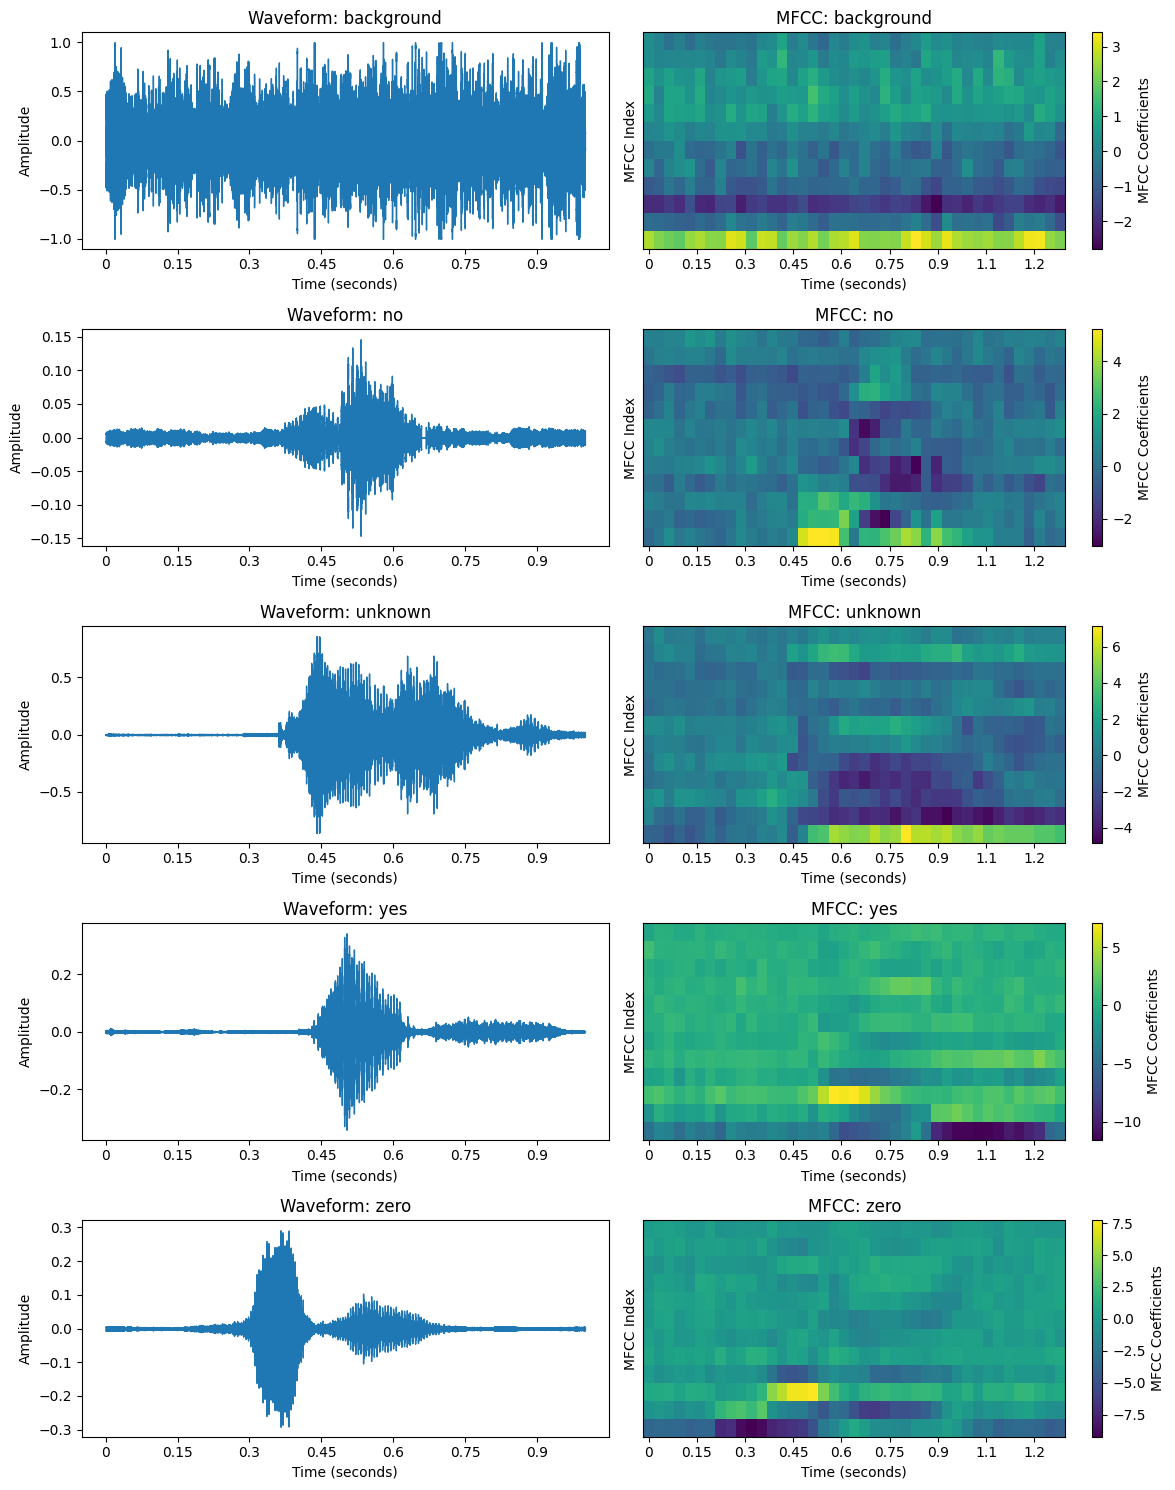
\includegraphics[width=1\linewidth]{Chapters/neuronska_mreza/dataset/mfcc.png} 
    \caption{Zvučni signali i pripadna matrica MFC koeficijenata}
    \label{pic:mfccpython}
\end{figure}

U ovom trenutku skupi podataka pripremljeni su za treniranje. Sljedeći korak je definicija 
strukture neuronske mreže.